\chapter{String Theory and M-Theory}

This chapter follows Leonard Susskind's lecture as a deliberate return to T-duality. The point is not merely that a small compact circle can masquerade as a large one, but that this statement can be sharpened into a worldsheet rule, translated into spacetime fields, and then pushed far enough to force new objects into the theory. The transcript is the primary guide throughout; the selected blackboard frames preserved by LazyingArt LLC and Video2Book are used only where they stabilize an equation, a diagram, or the grouping of fields on the board.

\section{Compactification, Closed Strings, and the Meaning of \(\sigma\)}

We begin in the simplest compactified setting. There is one large spatial direction, which we call \(x\), and one compact direction, which we call \(y\). To keep the notation close to the lecture, we write the compact identification as
\begin{equation}
y \sim y+r,
\end{equation}
where \(r\) is the distance around the compact cycle in the lecture's loose convention. In stricter notation one often separates radius from circumference, but here it is better to stay near the board and make the convention explicit.

The objects of interest at first are closed oriented strings. Thus the embedding coordinates are functions of worldsheet time \(\tau\) and worldsheet position \(\sigma\),
\begin{equation}
x=x(\tau,\sigma), \qquad y=y(\tau,\sigma), \qquad \sigma \sim \sigma+2\pi.
\end{equation}
The string is closed because it has no endpoints, and it is oriented because there is an intrinsic sense in which one can go around it one way or the other. Globally reversing every orientation would not change the theory, just as globally reversing all electric charges would not change the structure of electromagnetism; what matters is the relative comparison between two strings.

This orientation already constrains dynamics. When a closed string splits, the arrows must remain continuous. One cannot join or split strings arbitrarily; the local orientation data must be remembered by the process.

\subsection{Question \& Answer}

\paragraph{Question.} Is \(\sigma\) the same thing as going around the compact direction?

\paragraph{Answer.} No. This is the first obstruction in the lecture, and it is worth preserving exactly because the later formulas depend on it. The coordinate \(\sigma\) is only a label for points along the string. It runs from \(0\) to \(2\pi\) on every closed string, wound or unwound. A helpful picture is Susskind's rubber band: one may mark the molecules of the rubber band by names or by a parameter, but that labeling has nothing to do with whether the rubber band is wrapped around one's wrist.

The physical question of winding is a question about the embedding \(y(\tau,\sigma)\) in space. The parameter \(\sigma\) always goes once around the string itself. The map from the string into the compact direction may go around the \(y\)-circle zero times, once, twice, or in the opposite orientation. Those are different statements.

\section{Winding, Orientation, and Conserved Topology}

With that distinction in place, we can separate two kinds of closed strings. An unwound string does not wrap the compact direction at all. It is simply a closed string moving in a space with one compact coordinate. A wound string, by contrast, wraps the compact direction, and because the string is oriented there are two basic one-fold windings, opposite to each other.

The lecture does not introduce winding number by an abstract homotopy classification. Instead it is earned through joining and splitting processes. This is the right order. We first ask what can happen.

If two wound strings carry opposite winding, then the orientation-continuity rule allows them to join into a configuration that can be topologically deformed into a single unwound string. In that sense the pair can unwind:
\begin{equation}
(+1)+(-1)=0.
\end{equation}
If, on the other hand, two strings are wound the same way, then they cannot unwind. They can reconnect, but the result still carries total winding
\begin{equation}
(+1)+(+1)=2.
\end{equation}
The number of connected components can change; the total winding cannot.

This is the conservative heart of the discussion. A configuration with total winding \(100\) may appear as one string wound \(100\) times, or two strings wound \(50\) times each, or a hundred singly wound strings. These are dynamically related, but the total winding is not.

We therefore keep track of a conserved topological quantity \(W\). Positive and negative windings are distinguished by orientation, and \(W\) is additive under joining and splitting. The lecture repeatedly compares this with charge: one may not know absolutely whether a given orientation is the positive one, but one certainly knows whether two strings carry the same winding or the opposite winding.

\section{Momentum Modes, Winding Modes, and the Closed-String Form of T-Duality}

Now Susskind turns from pictures to spectra. An unwound string may carry momentum along the compact direction, and because that direction is periodic the compact momentum is quantized:
\begin{equation}
p_y \sim \frac{n}{r}, \qquad E_{\text{mom}} \sim \frac{n}{r},
\end{equation}
where \(n\in\mathbb{Z}\). In the lecture units the energy contribution from compact momentum is of the same scale as the compact momentum itself.

A wound string contributes energy in a different way. If the string tension is set to \(1\), then energy is proportional to length, and a string wound \(w\) times around the compact cycle carries energy
\begin{equation}
E_{\text{wind}} \sim w\,r.
\end{equation}

This already suggests the duality. If \(r\ll 1\), then
\begin{equation}
\Delta E_{\text{mom}} \sim \frac{1}{r} \gg 1, \qquad \Delta E_{\text{wind}} \sim r \ll 1.
\end{equation}
Momentum excitations are widely separated, while winding excitations are light. If \(r\gg 1\), the pattern reverses:
\begin{equation}
\Delta E_{\text{mom}} \sim \frac{1}{r} \ll 1, \qquad \Delta E_{\text{wind}} \sim r \gg 1.
\end{equation}
Thus the spectrum seen at small \(r\) can be re-read as the spectrum of a theory at large \(r\), provided we exchange momentum and winding. In the lecture normalization the crossover sits at
\begin{equation}
r=1.
\end{equation}

\begin{figure}[htbp]
\centering
\begin{tikzpicture}[x=0.85cm,y=0.65cm]
\draw[->] (0,0) -- (0,7.2);
\node at (0,7.8) {$r\ll 1$};
\node[rotate=90] at (-0.9,3.6) {$E$};
\node at (1.1,6.7) {momentum};
\foreach \yy/\lab in {0/0,2.8/1,5.6/2} {
  \draw (-0.25,\yy) -- (0.25,\yy);
  \node[right] at (0.3,\yy) {$n=\lab$};
}
\draw[->] (4,0) -- (4,7.2);
\node at (5.0,6.7) {winding};
\foreach \yy/\lab in {0/0,0.7/1,1.4/2} {
  \draw (3.75,\yy) -- (4.25,\yy);
  \node[right] at (4.3,\yy) {$w=\lab$};
}

\draw[->] (8,0) -- (8,7.2);
\node at (8,7.8) {$r\gg 1$};
\node at (9.1,6.7) {momentum};
\foreach \yy/\lab in {0/0,0.7/1,1.4/2} {
  \draw (7.75,\yy) -- (8.25,\yy);
  \node[right] at (8.3,\yy) {$n=\lab$};
}
\draw[->] (12,0) -- (12,7.2);
\node at (13.0,6.7) {winding};
\foreach \yy/\lab in {0/0,2.8/1,5.6/2} {
  \draw (11.75,\yy) -- (12.25,\yy);
  \node[right] at (12.3,\yy) {$w=\lab$};
}
\end{tikzpicture}
\caption{Schematic level spacings in the two dual regimes. When \(r\) is small, momentum modes are heavy and winding modes are light; when \(r\) is large, the roles reverse.}
\end{figure}

At the spectral level the exchange is therefore
\begin{equation}
n \leftrightarrow w, \qquad r \leftrightarrow \frac{1}{r}.
\end{equation}
But the lecture does not stop with the slogan. It now asks for a sharper mathematical statement.

The total compact momentum is the sum of the momenta of all the little bits of the string. Up to the lecture's suppressed normalization factors, this means
\begin{equation}
P_y \propto \int d\sigma\,\frac{\partial y}{\partial \tau}.
\end{equation}
The corresponding winding expression is written directly on the board:
\begin{equation}
W=\frac{1}{r}\int d\sigma\,\frac{\partial y}{\partial \sigma}.
\end{equation}
The lower formula is clearly visible in the lecture frame; the upper one is only partially legible on the board, so it is better to keep the momentum integral in its canonical transcript-backed form rather than pretend that every normalization on the board is readable.

\begin{figure}[htbp]
\centering

\includegraphics[width=0.72\textwidth]{lecture_10_figure_03.png}
\caption{Momentum and winding integrals on the board. The lower line is directly legible; the upper line fixes the structure of the momentum integral but not its full normalization.}
\end{figure}

\paragraph{Worked derivation.} For the simplest once-wound configuration, the lecture identifies \(\sigma\) with position around the compact direction:
\begin{equation}
\sigma \sim \frac{y}{r}.
\end{equation}
From this we get
\begin{equation}
\frac{d\sigma}{dy}=\frac{1}{r}.
\end{equation}
The winding expression may then be unpacked in the following way.
\begin{enumerate}
\item As \(\sigma\) goes once around the closed string, \(y(\sigma)\) goes once around the compact direction.
\item Therefore the total change in \(y\) over one circuit is \(\Delta y = w\,r\), after regularizing the lecture's loose period convention to \(y\sim y+r\).
\item Hence
\begin{equation}
W=\frac{1}{r}\int d\sigma\,\frac{\partial y}{\partial \sigma}
  =\frac{1}{r}\,\Delta y
  =\frac{1}{r}(w\,r)
  =w.
\end{equation}
\end{enumerate}
So the integral really does count winding.

\begin{figure}[htbp]
\centering
\begin{tikzpicture}[x=1cm,y=1cm]
\draw (0,0) ellipse (1,0.35);
\draw (-1,0) -- (-1,3);
\draw (1,0) -- (1,3);
\draw (0,3) ellipse (1,0.35);
\draw[->] (-1.7,0.2) -- (-1.7,1.8) node[left] {$y$};
\draw[->] (-0.7,-0.6) -- (0.8,-0.6) node[right] {$x$};
\draw[thick] (0.4,3.2) .. controls (1.0,2.4) and (-1.0,1.9) .. (-0.4,1.3)
            .. controls (0.9,0.7) and (-0.2,0.2) .. (0.4,-0.2);
\draw[->] (0.15,2.5) -- (0.45,2.25);
\node[right] at (0.55,2.45) {$\sigma$ increases};
\node at (3.4,1.5) {$y(\sigma+2\pi)=y(\sigma)+r$};
\end{tikzpicture}
\caption{A once-wound embedding. The parameter \(\sigma\) labels the string; winding is the statement that the embedding \(y(\sigma)\) changes by one period as \(\sigma\) goes once around the closed string.}
\end{figure}

\subsection{Question \& Answer}

\paragraph{Question.} How can an integral of a derivative measure winding instead of vanishing?

\paragraph{Answer.} Because the relevant quantity does not return to the same value as an ordinary single-valued coordinate would. The label \(\sigma\) returns to itself after one circuit, but the embedded coordinate \(y(\sigma)\) returns only modulo the compact identification. In the lecture this is said somewhat loosely as ``\(y\) changes by \(2\pi\).'' With the present normalization \(y\sim y+r\), the correct statement is that \(y\) changes by \(w\,r\). Therefore
\begin{equation}
\int d\sigma\,\frac{\partial y}{\partial \sigma}=\Delta y=w\,r,
\end{equation}
and division by \(r\) produces the winding number. The usual argument that the integral of a derivative vanishes is simply the wrong argument here.

This sharper viewpoint yields the worldsheet form of T-duality:
\begin{equation}
n \leftrightarrow w, \qquad r \leftrightarrow \frac{1}{r}, \qquad
\frac{\partial y}{\partial \tau} \leftrightarrow \frac{\partial y}{\partial \sigma}.
\end{equation}

\section{Worldsheet Derivatives and the Two Charge Sectors}

Once momentum and winding have both been written as worldsheet integrals, the lecture broadens the interpretation. These quantum numbers do not merely label states; they behave like charges. Opposite compact momenta attract, like compact momenta repel. Opposite windings attract, like windings repel. So the next question is unavoidable: what fields mediate these interactions?

For momentum, Susskind answers in Kaluza--Klein language. Start with gravity in five dimensions. The metric tensor has components
\begin{equation}
G_{MN}\longrightarrow \{G_{\mu\nu},\,G_{\mu 5},\,G_{55}\},
\end{equation}
where \(\mu,\nu\) are ordinary four-dimensional spacetime indices and \(5\) denotes the compact direction. The interpretation is immediate:
\begin{align}
G_{\mu\nu} &\quad \text{is the ordinary four-dimensional metric},\\
G_{\mu 5} &\quad \text{behaves as a four-dimensional vector } A_\mu,\\
G_{55} &\quad \text{behaves as a scalar } \phi.
\end{align}
The lecture loosely calls \(\phi\) a dilaton, but in the present discussion its role is more specific: it is the modulus controlling the size of the compact direction.

\begin{figure}[htbp]
\centering

\includegraphics[width=0.72\textwidth]{lecture_10_figure_04.png}
\caption{Five-dimensional metric components and their four-dimensional fields. The board emphasizes the identifications \(g_{\mu 5}\to A_\mu\) and \(g_{55}\to \Phi\).}
\end{figure}

Why does \(G_{\mu 5}\) play the role of an electromagnetic-type field? Because mixed metric components are sourced by momentum flow in the fifth direction. Thus the compact momentum quantum number becomes an electric-like charge for \(A_\mu\). The source of the effective vector field is precisely momentum around the compact circle.

Winding requires a second step. The lecture reopens the closed-string oscillator construction only schematically. The first level-matched massless sector is built from one left-moving and one right-moving oscillator,
\begin{equation}
a^i_{1,L}a^j_{1,R}|0\rangle.
\end{equation}
If one index is an ordinary spacetime index \(\mu\) and the other is the compact index \(5\), then we obtain vector-like states. Schematically one may form the combinations
\begin{equation}
a^\mu_{1,L}a^5_{1,R}|0\rangle \pm a^5_{1,L}a^\mu_{1,R}|0\rangle.
\end{equation}
The symmetric combination belongs to the metric sector and is associated with \(G_{\mu 5}\). The antisymmetric combination belongs to the Kalb--Ramond sector and is associated with \(B_{\mu 5}\). This second photon-like field couples to winding number.

Thus the lecture's closed-string picture of T-duality is already richer than the simple spectral exchange:
\begin{equation}
G_{\mu 5}\leftrightarrow B_{\mu 5}.
\end{equation}
Momentum and winding are not only exchanged as integers; the corresponding vector fields are exchanged as well. One sees why the lecture insists on the formal substitution
\begin{equation}
\frac{\partial y}{\partial \tau}\leftrightarrow \frac{\partial y}{\partial \sigma}:
\end{equation}
it is preparing the open-string argument still to come.

\section{Open Strings and the T-Duality Puzzle}

After the break the story is restarted on purpose. Closed strings have stable winding sectors; open strings do not. So if T-duality is truly an exact symmetry of string theory, what can it possibly mean for an open string?

The lecture first recalls the boundary condition for a free open string. At an endpoint there may be no net tension, for otherwise the endpoint would suffer infinite acceleration in the continuum limit. In the toy geometry this gives Neumann boundary conditions
\begin{equation}
\left.\frac{\partial x}{\partial \sigma}\right|_{\partial\Sigma}=0, \qquad
\left.\frac{\partial y}{\partial \sigma}\right|_{\partial\Sigma}=0.
\end{equation}
The first visible board line in the frame shows precisely the beginning of this statement.

\begin{figure}[htbp]
\centering

\includegraphics[width=0.72\textwidth]{lecture_10_figure_05.png}
\caption{Cylinder sketch with the beginning of the open-string boundary-condition equation. The final \(=0\) is supplied by the lecture itself rather than by the frozen board state.}
\end{figure}

The crucial point is that T-duality acts only on the compact direction. We do not touch the long coordinate \(x\); we only dualize \(y\). The lecture's rule is therefore
\begin{equation}
\frac{\partial y}{\partial \sigma}\leftrightarrow \frac{\partial y}{\partial \tau}.
\end{equation}
Applied at the endpoint, this transforms the free-endpoint condition into
\begin{equation}
\left.\frac{\partial y}{\partial \sigma}\right|_{\partial\Sigma}=0
\quad \xrightarrow{\,T\,} \quad
\left.\frac{\partial y}{\partial \tau}\right|_{\partial\Sigma}=0.
\end{equation}

\begin{figure}[htbp]
\centering
\begin{tikzpicture}[x=1cm,y=1cm]
\draw (0,0) ellipse (1,0.35);
\draw (-1,0) -- (-1,2.8);
\draw (1,0) -- (1,2.8);
\draw (0,2.8) ellipse (1,0.35);
\draw[->] (-0.7,-0.6) -- (0.8,-0.6) node[right] {$x$};
\draw[->] (-1.6,0.2) -- (-1.6,1.5) node[left] {$y$};
\draw[thick] (-0.3,2.2) .. controls (0.6,1.8) and (-0.2,1.0) .. (0.6,0.5);
\fill (-0.3,2.2) circle (0.05);
\fill (0.6,0.5) circle (0.05);
\node at (3.6,1.3) {$\left.\partial_\sigma y\right|_{\partial\Sigma}=0$};
\node at (3.6,0.7) {$\downarrow\ T$};
\node at (3.6,0.1) {$\left.\partial_\tau y\right|_{\partial\Sigma}=0$};
\end{tikzpicture}
\caption{The compact direction is the only one dualized. The Neumann condition becomes a Dirichlet condition in that direction.}
\end{figure}

\subsection{Question \& Answer}

\paragraph{Question.} Why does T-duality turn a free endpoint into a fixed one?

\paragraph{Answer.} Because a vanishing \(\tau\)-derivative at the endpoint means the endpoint is not moving in the dualized direction. Before duality the endpoint is free because its spatial derivative vanishes: there is no net stretching at the end. After duality the object that vanishes is the time derivative in the compact direction, so the endpoint stays at a fixed value of \(y\). What was a free endpoint in the original description becomes a pinned endpoint in the dual description.

This is the decisive turn of the lecture. T-duality is no longer only a statement about spectra or about field identifications. It has become a statement about what kinds of objects must exist in the theory.

\section{Dirichlet Boundary Conditions and the Emergence of D-Branes}

If the endpoint is fixed in the compact direction, fixed by what? The lecture insists on the answer: there must be an object in the theory that can hold the endpoint in place. That object is a D-brane, where \(D\) stands for Dirichlet.

The important point is that the D-brane is not inserted as decoration. It is discovered by asking that open strings and T-duality coexist consistently. One begins with free open strings and ends with a dual description in which the endpoints are nailed down. The mathematics therefore demands something that can act as an anchor.

That anchor cannot be an absolutely rigid, immovable blemish in space. Nothing in the argument singles out one point rather than another, so the brane must be movable. And because we are in a relativistic theory, it must also be bendable. The lecture lingers on this because it matters physically: these are not mere boundary markers, but dynamical objects.

The dimensionality count is simple and powerful. In ten-dimensional string theory there are nine spatial dimensions. If \(k\) spatial directions are fixed by Dirichlet conditions, then the endpoint remains free to move in the remaining
\begin{equation}
p=9-k
\end{equation}
spatial directions. The locus on which the endpoint can move is therefore a D\(p\)-brane.

The lecture explains this through the tabletop analogy. In ordinary three-dimensional space:
\begin{itemize}
\item one constraint leaves a two-dimensional plane,
\item two constraints leave a one-dimensional line,
\item three constraints leave a point.
\end{itemize}
Exactly the same logic works in nine spatial dimensions.

\begin{figure}[htbp]
\centering
\begin{tikzpicture}[x=2cm,y=1cm]
\node at (0,1.2) {one constraint};
\draw (-0.7,0) -- (0.7,0);
\node at (0,-0.5) {plane};

\node at (2.5,1.2) {two constraints};
\draw (2.5,-0.7) -- (2.5,0.7);
\node at (2.5,-1.0) {line};

\node at (5,1.2) {three constraints};
\fill (5,0) circle (0.05);
\node at (5,-0.5) {point};
\end{tikzpicture}
\caption{The tabletop counting argument used in the lecture. Each Dirichlet constraint removes one independent direction of endpoint motion.}
\end{figure}

Thus repeated T-dualities generate the familiar ladder
\begin{equation}
\text{D}8,\ \text{D}7,\ \text{D}6,\ \dots,\ \text{D}0.
\end{equation}
The space-filling end of the story should be handled carefully. A D9-brane is simply the case in which open strings are free to move through all spatial directions, so in that sense ordinary open-string theory may be regarded as open strings living on a space-filling brane.

The lecture also makes one further conceptual move. Although the T-duality argument begins with compact directions, one may shrink a compact circle so far on one side of the duality that on the other side it becomes effectively noncompact. In this way the conclusion is broadened: D-branes can extend along noncompact directions as well. They are not confined to some hidden compact corner of the geometry.

\section{Physics on Branes: Gauge Fields, Color, and Monopoles}

Now the lecture spends its payoff. What do these objects do?

Begin with one brane. Low-energy open strings ending on that brane behave like particles confined to its worldvolume. Their splitting and joining look like particle processes, and in the low-energy limit one obtains an ordinary quantum field theory on the brane. With one brane the lecture reads this as a QED-like sector: strings with both ends on the brane behave like photon-like excitations on the brane, while strings with only one end on the brane behave like charged matter.

With several parallel branes, the story becomes more interesting. The lecture names three of them Red, Green, and Blue. An oriented open string can begin on one brane and end on another, so it carries an ordered pair of labels. That is exactly the sort of bookkeeping one needs for gluon-like states.

\begin{figure}[htbp]
\centering
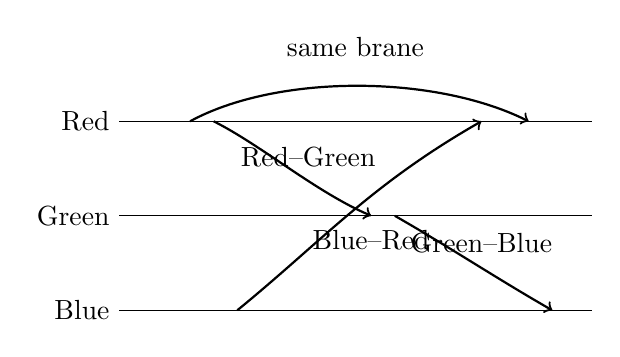
\begin{tikzpicture}[x=1cm,y=1cm]
\draw (0,2.4) -- (6,2.4);
\draw (0,1.2) -- (6,1.2);
\draw (0,0) -- (6,0);

\node[left] at (0,2.4) {Red};
\node[left] at (0,1.2) {Green};
\node[left] at (0,0) {Blue};

\draw[->,thick] (0.9,2.4) .. controls (2.0,3.0) and (4.0,3.0) .. (5.2,2.4);
\draw[->,thick] (1.2,2.4) .. controls (1.8,2.1) and (2.5,1.5) .. (3.2,1.2);
\draw[->,thick] (3.5,1.2) .. controls (4.2,0.8) and (4.8,0.4) .. (5.5,0);
\draw[->,thick] (1.5,0) .. controls (2.6,0.9) and (3.2,1.6) .. (4.6,2.4);

\node at (3.0,3.35) {same brane};
\node at (2.4,1.95) {Red--Green};
\node at (4.6,0.85) {Green--Blue};
\node at (3.2,0.9) {Blue--Red};
\end{tikzpicture}
\caption{Parallel branes with oriented open strings. Ordered endpoints furnish the pair of color labels that mimic the gluon sector on the brane stack.}
\end{figure}

The lecture does not try to reconstruct the full Yang--Mills formalism from scratch. Instead it follows the string processes. If one has a Red--Green string and a Green--Blue string, their compatible endpoints can join and produce a Red--Blue string. These are precisely the kinds of combinatorial rules that one associates with nonabelian gauge bosons. One linear combination can lift off the brane stack, which is why the lecture remarks that one finds eight gluons rather than nine naive color-pair states.

Quarks are represented differently. A quark carries one color label, not a color and an anticolor. In the brane picture this means a string with only one end attached to the color brane stack; the other end extends elsewhere, either to a distant brane or effectively off to infinity. A quark and an antiquark can annihilate when their compatible ends meet. Two quarks cannot.

With a single brane the resulting worldvolume theory is QED-like; with a stack of several branes it becomes Yang--Mills-like; and the lecture's historical point is that none of this was the starting assumption. It was discovered by following the consistency conditions imposed by T-duality.

The final step is the magnetic one. Besides the ordinary fundamental strings, the theory also contains D-strings, which are heavier one-dimensional D-branes. A D-string can end on a D3-brane. If an ordinary string endpoint on a D3-brane behaves like an electric charge, then the endpoint of a D-string behaves as its magnetic dual:
\begin{equation}
\text{D-string ending on a D3-brane} \quad \longrightarrow \quad \text{magnetic monopole}.
\end{equation}
Because the D-string is much heavier than the fundamental string, the corresponding monopole is much heavier than the electric charge. The lecture does not derive the full monopole dynamics; it uses the example to emphasize how naturally electric and magnetic sectors appear once D-branes are present.

\section{Summary}

The lecture has a very tight arc. We start with a compact circle and closed oriented strings. That gives two sectors, momentum and winding, with energies \(n/r\) and \(wr\). Their spectra become indistinguishable after the exchange
\begin{equation}
n\leftrightarrow w, \qquad r\leftrightarrow \frac{1}{r},
\end{equation}
and the indistinguishability becomes sharper once momentum and winding are written as
\begin{equation}
P_y \propto \int d\sigma\,\frac{\partial y}{\partial \tau},
\qquad
W=\frac{1}{r}\int d\sigma\,\frac{\partial y}{\partial \sigma}.
\end{equation}
At that point T-duality is the exchange of \(\partial_\tau y\) with \(\partial_\sigma y\), together with a corresponding exchange of the vector fields that couple to momentum and winding.

Then the decisive move is made. Apply the same duality to open strings, and Neumann boundary conditions become Dirichlet ones. Endpoints that were free are now fixed. The theory therefore requires objects that can anchor string endpoints: D-branes. Once those objects are allowed, open strings on them produce lower-dimensional gauge theories, stacks of branes produce color-labelled gauge bosons, and D-strings ending on D3-branes produce magnetic monopoles. The lecture closes exactly where it intended to close: T-duality was not an isolated curiosity, but one of the routes by which string theory discovered its own deeper structure.